\section{Implementation}
\label{sec:impl}
Our approach to the DNS rebinding attack is derived from a standard time-varying attack, which can potentially take several minutes based on browser implementation of DNS Pinning. We discovered a previously undocumented variation which takes on the scale of tens of seconds. Instead of waiting for the pinned entries to expire, we flood the DNS cache with enough invalid entries to remove valid entries from the list. We built on this idea and provided the attacker with a seamless browsing experience on the victim's internal server, as shown in Figure \ref{fig:firedrill1}. The next step is to retrieve the data from the victim's server (similar to existing scraping methods). Then we will allow the attacker to click links, take actions, and submit forms by sending the data to the victim's browser,which is acting as a proxy. The JavaScript on the browser then forwards the appropriate request to the server.

\begin{figure}[h]
\centering
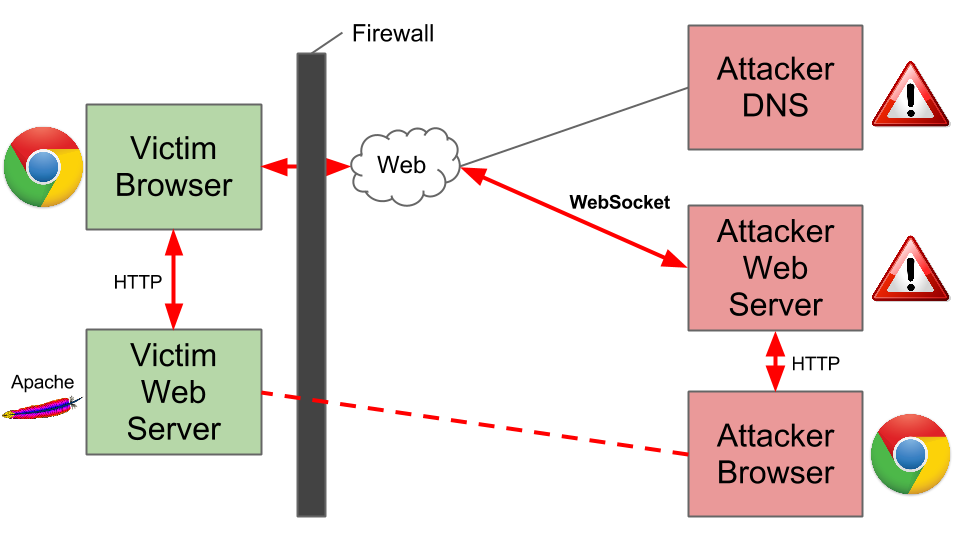
\includegraphics[width=0.8\columnwidth]{firedrill1.png}
\caption{\textbf{FireDrill Attack Overview.} When a victim accesses the attacker's web server, a malicious Javascript payload is delivered and runs on the victim's browser. It then issues a large batch of DNS request to flood victim's DNS table and rebind the original domain name to the IP address of victim's web server. The victim's browser then becomes a proxy between the internal websites and the attacker's browser. The attacker can navigate it as he would any other website.}
\label{fig:firedrill1}
\end{figure}

\subsection{Malicious DNS server}
Our system consists of a custom DNS server authoritative for the domain name takenoteswith.us. The DNS server keeps track of DNS requests and their source IP address. When the DNS server sees a request for the first time, it returns a IP address \textbf{54.224.61.225}, which is the address of our web server. If the DNS server has seen the DNS requests from the same IP address twice, it knows that this DNS requests is initiated by the rebinding script. At this time, the the malicious DNS server will return an IP address of \textbf{127.0.0.1}, or whichever IP address the attacker wants to target.

\subsection{Rebinding based on DNS table flooding}
To remove a pinned entry from the DNS entry table, we use a DNS flooding technique. In current implementations of Chrome, all the domain names that are in the same level have the same priority. For this reason, we set our malicious URL (which the victim must request) to \textbf{n1.takenoteswith.us}.
We then flood the DNS table using DNS records from \textbf{n2.takenoteswith.us} to \textbf{n120.takenoteswith.us}. In this case, we assume the browser's DNS table size is 100. The number of invalid DNS requests are slightly more than 100 here because we want to speed up the process by eliminating the tail effects.

The careful readers may notice that the request should not have completed since it disobeys the same-origin policy. However, the Chrome browser will still put the invalid entry in the DNS cache table and treat them with the same priority. 

\subsection{Malicious Javascript proxy}
The malicious Javascript proxy will be run on the victim's browser. It builds a WebSocket connection to the attacker's webserver and receives proxy commands from it. The commands from the webserver have three fields, the \textbf{method} field is used to specify whether an HTTP \emph{post} or \emph{get} request should be forwarded. The \textbf{url} field specify the target of the request. The \textbf{args} field contains the arguments of the request.

The response from the JavaScript proxy to the server must take additional step to maintain data integrity. Apart from plain HTML, sometimes the attacker wants to access binary data such as image and audio files. In this case, the proxy has to put the HTTP headers('content-type', specifically) into the response so that the attacker's browser knows how to parse and encode it. If the response is compressed, the JavaScript is required to decompress it. In this case, the HTTP header field 'content-length' should be changed accordingly. Lastly, if the response contains binary data, the JavaScript must encode it using base64 so that it can be transmitted in a JSON object. 

\subsection{Attacker's interface}
When a victim is connected, a new session is created and the attacker will be notified via both a web interface and e-mail. The attacker can access the interactive session using his browser as we would with regular websites. The notifications contain links which the attacker can click to easily begin the session with the victim's web server.

When the attacker requests a web object, it sends a request to his web server which is connected to the victim's browser via the persistent WebSocket connection. The web server will spawn a thread to handle the request. The thread will then forward the request to the JavaScript proxy, sleep and wait for the request then wake up again when the response from the proxy is available. The thread then decodes the response, rebuilds the HTTP header, then forwards it back to the attacker's browser, thus completing the request reponse.
